\documentclass[journal, a4paper]{IEEEtran}

\usepackage{graphicx}
\usepackage{caption}
\usepackage{subcaption}
% some very useful LaTeX packages include:

%\usepackage{cite}
\usepackage{graphicx}
\usepackage{amsmath,eqparbox,booktabs,xparse}
\usepackage{smartdiagram}
\usetikzlibrary{quotes}
%\usepackage{psfrag}   
%\usepackage{subfigure}
\usepackage{neuralnetwork}
\usepackage{url}        % Written by Donald Arseneau
%\usepackage{stfloats}  % Written by Sigitas Tolusis
\usepackage{xcolor}
%\interdisplaylinepenalty=2500
\usepackage{listings}

\lstset{basicstyle=\ttfamily, keywordstyle=\bfseries}
\usetikzlibrary{arrows.meta, positioning}
\tikzset{%
    block/.style = {draw=gray, rectangle, thick,
        minimum height=6em, text width=4em, align=center}
}

\makeatletter
\NewDocumentCommand{\eqmathbox}{o O{c} m}{%
  \IfValueTF{#1}
    {\def\eqmathbox@##1##2{\eqmakebox[#1][#2]{$##1##2$}}}
    {\def\eqmathbox@##1##2{\eqmakebox{$##1##2$}}}
  \mathpalette\eqmathbox@{#3}
}
% Your document starts here!
\begin{document}

% Define document title and author
	\title{RocketDeepL \\ \textit{\Large{A mini deep learning framework}}}
	\author{Francis \textbf{Damachi} - Costanza \textbf{Volpini}}
	\markboth{Project 2 - Deep Learning EE559 - EPFL}{}
	\maketitle
	
\begin{abstract}
In the last few years, Neural Networks have proved to be one of the most effective solutions to tackle a wide range problems (e.g. image and speech recognition, language processing). The aim of this project is to design a multi-layer perceptron capable using the standard math library and the basic tensor operations of Pytorch.
\end{abstract}

\section{Introduction}
\label{sec:intro}
A simple neural networks is composed by an input layer, a series of hidden layers and an output layer (see Fig. \ref{fig:neuralnet}). Each layer has a certain number of neurons (nodes) each of which processes all the features computed by the previous layer; the nodes of the input layer process the features of the input samples. In a classification task, the number of nodes of the last layer is usually equal to the number of classes to be detected.

\begin{figure}[h]
    \centering
\begin{neuralnetwork}[height=5, nodespacing=10mm, layerspacing=23mm]
		\newcommand{\nodetextclear}[2]{}
		\newcommand{\nodetextx}[2]{$x_#2$}
		\newcommand{\nodetexty}[2]{$y_#2$}
		\inputlayer[count=2, bias=false, title=Input\\layer, text=\nodetextx]
		\hiddenlayer[count=5, bias=false, title=Hidden\\layer, text=\nodetextclear] \linklayers
		\hiddenlayer[count=5, bias=false, title=Hidden\\layer, text=\nodetextclear] \linklayers
		\outputlayer[count=2, title=Output\\layer, text=\nodetexty] \linklayers
	\end{neuralnetwork}
	\caption{General neural network with two hidden layers.}
    \label{fig:neuralnet}
	\end{figure}
\textit{Perceptron} is the key concept of a neural network, it is a linear classifier (binary) which decides whether or not each input belong o a certain class. Some \textit{parameters} are then introduced so that the obtained parametric function can be optimized in order to obtain the correct output for each input sample. 
The output of the network is unbounded and is obtained by computing $\sum_i w_i x_i + b$ where $w_i$ is a weight and $x_i$ is an input feature. The \textit{bias} $b$ allows to translate the linear function that would otherwise intersect the origin of the axes. Then, the classification is obtained by comparing this output with respect of a threshold which is usually set to $0$. Formally, the output is computed as follows:
$$ \mbox{output} = \begin{cases}
     & 1 \;\; \mbox{if} \;\; \sum_i w_i x_i + b \geq 0 \\
     & 0 \;\; \mbox{otherwise}
\end{cases}$$
To make the neural network also learn to discriminate non-linearly separable samples, non-linearities have to be introduced. In particular, \textit{activation layers} (see Sec. \ref{sec:activation}) are used after each linear layer, i.e. the output is obtained by
$ \sigma (w x + b)$. Since $\sigma$ is a non-linear function, it allows the network to approximate more complex function and, usually, guarantee a better accuracy.
\\ \\
In our implementation, weights and bias are initialized from a uniform random distribution and the values are defined by $[-stdv, +stdv]$ (where $stdv = 1 / \sqrt{output\_layer}$). In case of a binary classification, after this random initialization, we expect our neural network to achieve an accuracy of around $50\%$. 
The main core of the project is to define and implement the learning algorithm. First of all, we apply the \textit{forward pass}, then \textit{backward pass} and, finally, we update all the \textit{parameters}.
\begin{enumerate}
    \item \textit{Forward pass}:
computes values from inputs to output.
 \item \textit{Backward pass}:
start from the computed loss and performs backpropagation by applying recursively the \textit{chain rule} in order to compute all the gradients of the loss with respect of the various parameters of the network. The loss function is used in order to detect how much the output differs from the expected one.
\begin{figure}
    \centering
    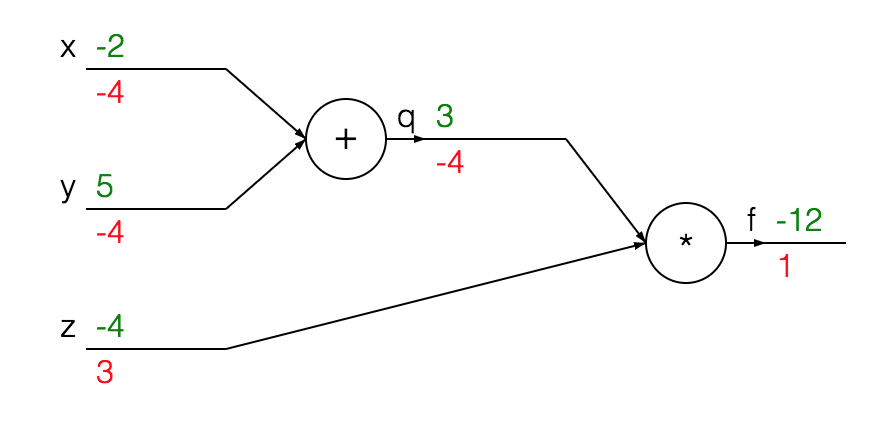
\includegraphics[width=0.8\linewidth]{backandfor.png}
    \caption{Example of forward and backward passes. The first is represented in green and the second in red. \cite{reference0}}
    \label{fig:my_label}
\end{figure}
\item \textit{Update parameters}:
to minimize the train loss we update all the parameters using the gradients computed during the \textit{backward pass}. In particular, all the parameters are updated in the opposite direction of their corresponding gradient.
\end{enumerate}
In the following sections we will analyze deeply the architecture and we will provide a description of the structure of the code of our framework.
Let's define $\left[ \frac{\partial l}{\partial s^{(l)}}\right] = \left[ \frac{\partial l}{\partial x^{(l)}}\right] \odot \sigma ' (s^{(l)})$.
\\
\\
\begin{tabular}{*{2}{l} }
  \toprule
  \textbf{Name} & \textbf{Formula} \\
  \midrule
  \raisebox{-.01\normalbaselineskip}[0pt][0pt]{Forward pass} &
    $x^{(l)} = \sigma (w^{(l)}x^{(l-1)} + b^{(l)})$\\
  \raisebox{-.01\normalbaselineskip}[0pt][0pt]{Backward pass} &
    $\left[\frac{\partial l}{\partial w^{(l)}}\right] =\left[\frac{\partial l}{\partial s^{(l)}} \right] \left( x^{(l-1)}\right)^T$, $\left[\frac{\partial l}{\partial b^{(l)}}\right] = \left[\frac{\partial l}{\partial s^{(l)}}\right]$\\
  \bottomrule
\end{tabular}

\section{Data set}
\label{sec:dataset}
The data used for training and testing is composed by $1000$ points sampled distributed in range $[0, 1]^2$, points outside the radius $\frac{1}{\sqrt{2\pi}}$ are labelled with 0 target, otherwise 1 (See Fig. \ref{fig:generated-dataset}).
\begin{figure}[!h]
    \centering
    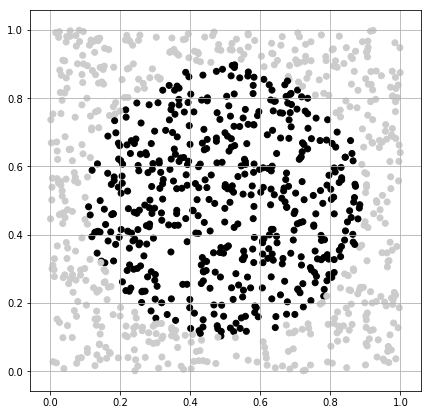
\includegraphics[width=0.8\linewidth]{gen.png}
    \caption{Points are sampled distributed in range $[0, 1]^2$. Points labelled with 0 are shown in gray, else in black.}
    \label{fig:generated-dataset}
\end{figure}
The labels are encoded using a one-hot encoding scheme.
The code that provide the generation of the dataset can be found in the file \texttt{generator\_training\_set.py}.

\section{Implementation}
We have decided to use a modular approach in order to make possible to modify or expand it. Backpropagation has been implemented storing all the information of the graph, so that each node keeps track of its input other than calculating its result. Then, to compute the derivative of its input wrt the loss, we can just compute the gradient of the input wrt the result of the node and apply the chain rule to update the gradient obtained by the next operation. The computed gradient is then passed to the inputs. The forward pass just computes the output and return it, instead, for the backward pass each node receive the gradient from its output (\texttt{gradientwrtoutput} parameter in the code method) and it multiplies this value with the gradient of the output with respect to each inputs (\texttt{grad\_w} and \texttt{grad\_b} fields). Each gradient is then accumulated in the gradient field of the corresponding parameter (\texttt{grad\_w} field). The structure used to define the \texttt{module} class requires 3 methods \texttt{forward}, \texttt{backward} and \texttt{params}, this is used to implement the basic layers; e.g. linear and activation layers.

\section{Code structure}
\label{sec:codestruc}
In this section we will describe the content of the files in the library \textit{RocketDeepL}.
\begin{itemize}
    \item \texttt{relu.py}: activation class that implements the ReLU operation (non-linear function).
    \item \texttt{sequential.py}: this class is used to handle different classes. As input it takes a list of layers that compose the neural net.
    \item \texttt{sgd.py}: optimizer class that it is initialized with a \textit{learning step} parameter.
    \item \texttt{tanh.py}: activation class that implements the hyperbolic tangent operation (non-linear function).
    \item \texttt{l\_mse.py}: class that implements the mean square error.
    \item \texttt{layers.py}: it implements the class Linear that is a wrapper of two operation: sum of biases and multiplication of weights ($y = xw + b$).
    \item \texttt{module.py}: abstract class \textit{Module} containing the basic methods.
\end{itemize}


\section{Activation layer}
\label{sec:activation}
We have implemented two activation layers; the first use \textit{ReLU} as activation function, the second one \textit{tanH} function. 
As explained in Section \ref{sec:intro}, the activation functions have been proved to be essential to approximate more complex functions and guarantee a good accuracy.
\begin{itemize}
    \item \textit{ReLU} is one of the most used activation function ($f(x) = max(0, x)$), its output is defined in an interval $[0, \infty )$. However, when the input smaller than 0 then also all the gradient are 0s which lead to a null update of the model parameters. This causes a bad train of the model. File: \texttt{rocket\_deepl/core/activations/relu.py}
    \item \textit{tanH} is an activation function ($f(x) = \frac{sinh(x)}{cosh(x)} = \frac{e^{2x} - 1}{e^{2x} + 1}$), its output is defined in the interval $(-1, 1)$. This activation is is differentiable on all R. It is mainly used for a binary classification. It maps negative inputs values close to -1 and positive inputs to values close to 1. File: \texttt{rocket\_deepl/core/activations/tanh.py}
\end{itemize}
% should be cite this? https://towardsdatascience.com/activation-functions-neural-networks-1cbd9f8d91d6


\section{Learning with gradient descent}
\label{sec:learning}
\textit{Gradient descent} is the algorithm that we have used in order to minimize the mean square error (\textit{MSE}). The latter is defined as:
$$\mathcal{L}(w, b) = \frac{1}{2n} \sum_x ||y(x) - a||^2 $$
where $y$ represents the model which depends on the weights $w$ and biases $b$ that are the parameters that we want to optimize in order to minimize the cost function; $n$ is the total number of training inputs and $a$ is the vector of correct outputs corresponding to $x$. In particular, to speed the treaining process we have decided to use a \textit{stochastic gradient descent} algorithm. 
The update of a parameter $p$, will be expressed as 
$ p = p + \eta \nabla \mathcal{L} (p)$.
\cite{reference1}

The implementation of SGD can be found in the file \texttt{rocket\_deepl/optimizer/sgd.py}.

\section{Linear layer}
\label{sec:linearl}
The parameters that are trainable in a  \textit{fully connected layer} are the weights and biases. However, it is important to notice that these values are initialized from an uniform random distribution, in a range $[-std, std]$, that gives a starting point to our stochastic gradient descendent. It is expressed as follow,
$$ y = xW + b\;\;\mbox{where}\;\;y\in R^{1xD}\mbox{,} \;\; x \in R^{1xM}\mbox{,}\;\;$$$$ W\in R^{MxD}\;\;\mbox{and}\;\;b \in R^{1xD} $$

All the corresponding implementation can be found in the file \texttt{rocket\_deepl/core/layers.py}.

\section{Comparison of Model}
% Almost same result
% Accuracy
% compare with logistic
{\Huge{TODO: compare with logistic!!!!!!!}}

% \section{Bonus}
\section{Result}
In this report, we have designed a multi-layer perceptron (MLP) capable using the standard math library and the basic tensor operations of Pytorch. We have trained it using stochastic gradient descent (SGD). The result obtained are really close to the one of the official pytorch \textit{nn library}.

We have tried our deep learning framework with the following specifics (see Fig. \ref{fig:res}) on the dataset showed in Section \ref{sec:dataset}:
\begin{itemize}
    \item \textit{inputs}: two input units (e.g. \textit{x} and \textit{y}).
    \item \textit{outputs}: two output units.
    \item \textit{layers}: 3 hidden layers of 25 nodes.
\end{itemize}
{\Huge{check image - layers}}
\begin {figure}[h!]
\centering
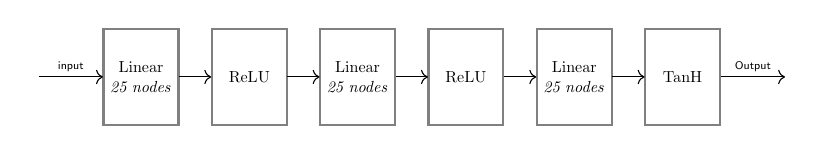
\begin{tikzpicture}[node distance = 0.5cm,
    every edge quotes/.append style={sloped, font=\sffamily\scriptsize, auto},
    scale=0.58,transform shape
  ] 
    \node (first) {};
    \node [block, right=40pt of first] (A) {Linear \\ \textit{25 nodes}}; 
    \node [block, right=20pt of A] (B) {ReLU}; 
    \node [block, right=20pt of B] (C) {Linear \\ \textit{25 nodes}}; 
    \node [block, right=20pt of C] (D) {ReLU}; 
    \node [block, right=20pt of D] (E) {Linear \\ \textit{25 nodes}}; 
    \node [block, right=20pt of E] (F) {TanH}; 
    \node [right=40pt of F] (out) {};
    \draw[->]
    (first) edge ["input"] (A)
  (A) edge (B) (B) edge (C) (C) edge (D) (D) edge (E) (E) edge (F) (F) edge ["Output"] (out) ;
\end{tikzpicture}
\caption{Structure of model that we have used for testing.}
\label{fig:res}
\end{figure}
The input and the hidden layer are followed by a ReLU while the output layer followed the \textit{TanH}. This allows to obtain a bounded output (in range $[-1, 1]$) which makes it possible to avoid a huge penalization of large positives and negatives values when using \textit{MSE} (the loss and accuracy are shown in Fig. \ref{fig:plot}). This is crucial in the case we have a binary classification.
\begin{figure}[!h]
    \centering
    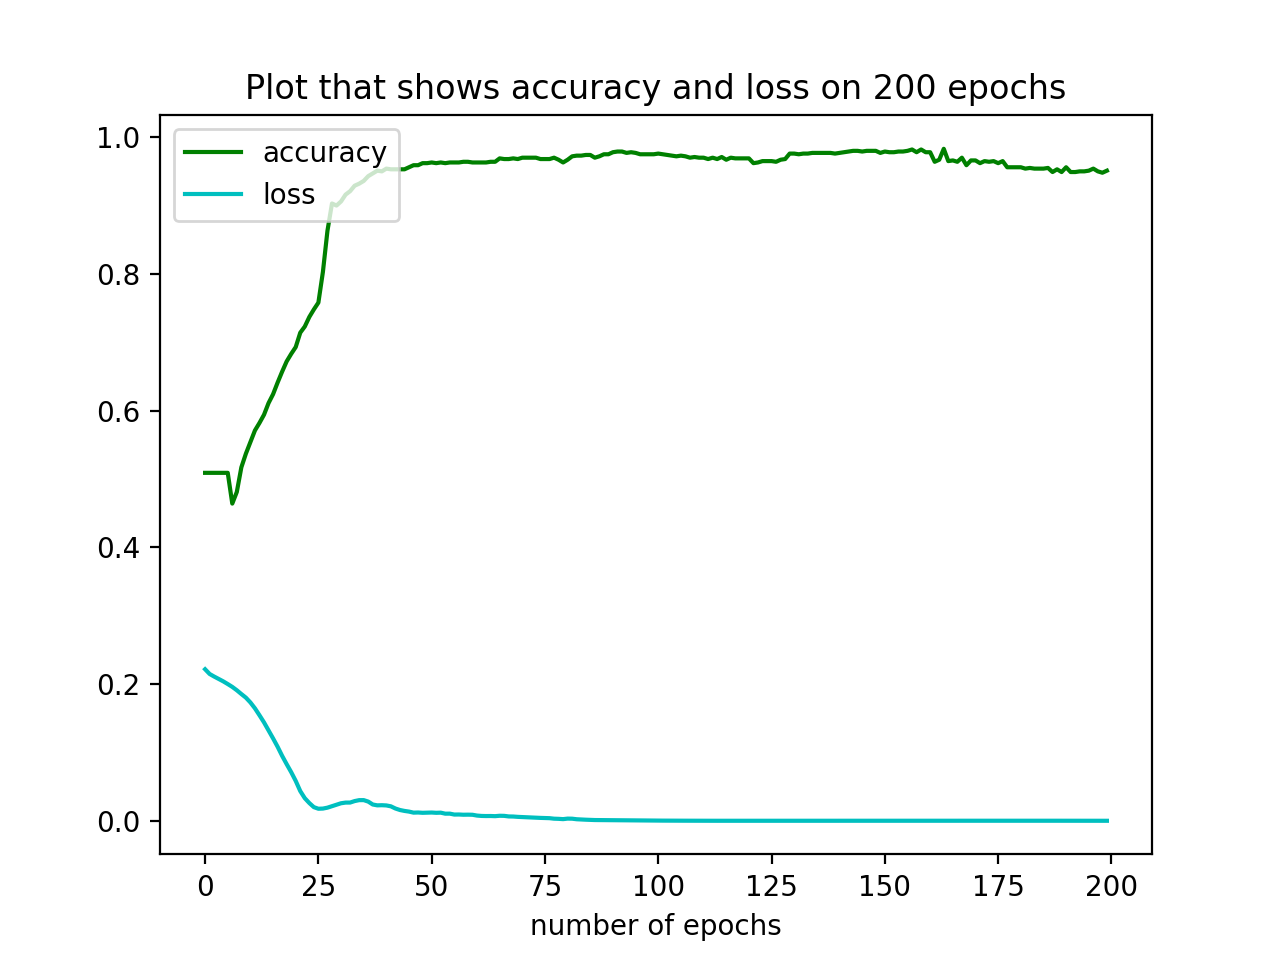
\includegraphics[width=0.9\linewidth]{Figure_1.png}
    \caption{Results obtained training the model of Fig. \ref{fig:res}}
    \label{fig:plot}
\end{figure}
The corresponding code, generate the model in our framework.
\begin{lstlisting}[language=Python]
model = Sequential([Linear(2, 25), ReLU(),
Linear(25,25), ReLU(), Linear(25,25), ReLU(),
Linear(25, 2), tanH()])
\end{lstlisting}
Training this model with $200$ epochs we got an accuracy of $96.2\%$ and $38$ miss-predictions.

% Now we need a bibliography:
\begin{thebibliography}{999}

	%Each item starts with a \bibitem{reference} command and the details thereafter.
	\bibitem{reference0}
    	Notes of CS231 Convolutional Neural Networks for Visual Recognition.
    	\url{https://cs231n.github.io/optimization-2}
	
	\bibitem{reference1}
	    Neural networks and deep learning, Michael Nielsen.
	    
    \bibitem{reference2}
    Notes of course Deep Learning (EE-559), Prof. François Fleuret.

\end{thebibliography}

% Your document ends here!
\end{document}